%====================================================================================
\section{Funciones de bienestar social}
%====================================================================================

\begin{frame}{Concepto de Función de Bienestar Social}
	\begin{itemize}
		\item La función de bienestar social $(FBS)$ mide el bienestar de la sociedad como una función de la utilidad de los individuos.
		
		\item Permite:
				\begin{itemize}
					\item Establecer un orden social de los posibles estados ``productos de diferentes políticas''.
					\item que se hagan comparaciones entre diferentes políticas y que se escoja la política que maximiza el bienestar de la sociedad.
				\end{itemize}
	\end{itemize}
\end{frame}
%------------------------------------------------
\begin{frame}{Juicios de valor adicionales}
	\begin{enumerate}
		\item El bienestar de la sociedad aumenta si la utilidad de un agente económico aumenta y la de los otros permanece igual.
				$$\frac{\partial W}{\partial U_A} > 0$$
	\end{enumerate}
\end{frame}
%------------------------------------------------
\begin{frame}{Juicios de valor adicionales}
	\begin{enumerate}[2]
		\item Si después de un cambio, un individuo empeora, entonces otro individuo tiene
		que estar mejor para conservar constante el nivel de bienestar de la sociedad.
				\begin{gather*}
					\frac{\partial W}{\partial U_A}dU_A + \frac{\partial W}{\partial U_B}dU_B = 0 \\[0.4cm]
					\frac{dU_A}{dU_B}  = -\left(\frac{\partial W/\partial U_A}{\partial W/\partial U_B} \right) < 0
				\end{gather*}
	\end{enumerate}
\end{frame}
%------------------------------------------------
\begin{frame}{Juicios de valor adicionales}
	\begin{enumerate}[3]
		\item Si un individuo tiene un nivel alto de utilidad y el otro individuo tiene un nivel bajo de utilidad, la sociedad estará dispuesta a sacrificar parte de la utilidad del primer individuo para incrementar la utilidad del segundo individuo.
	\end{enumerate}

	\begin{figure}[!h]
		\centering
		\hspace{1.2cm}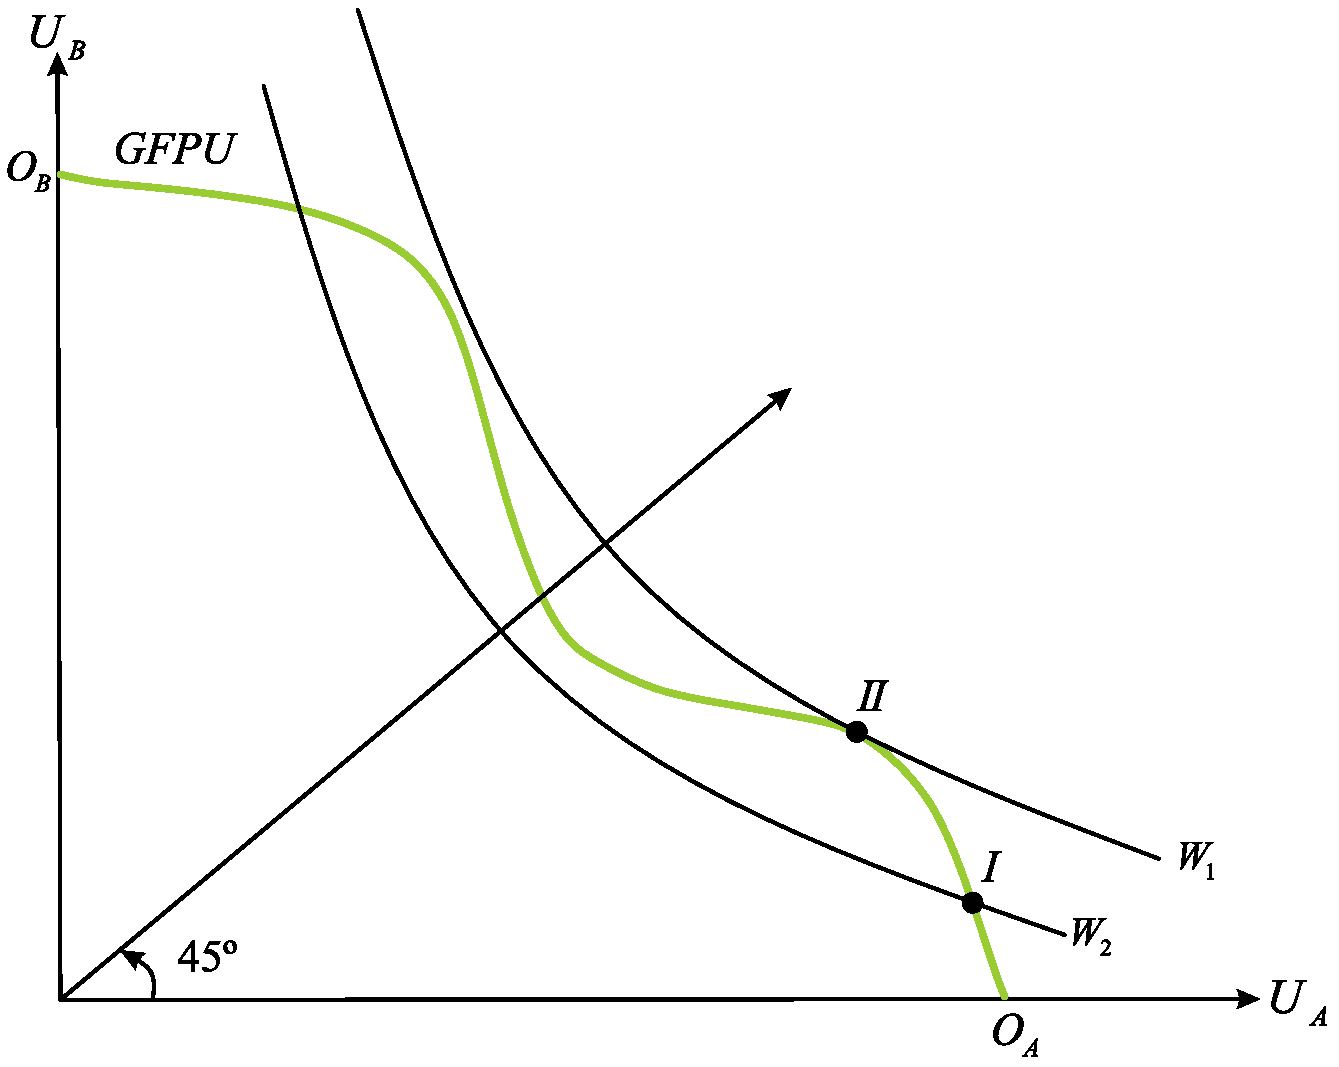
\includegraphics[width = 0.6\linewidth]{figures/fig_08.pdf}
	\end{figure}
\end{frame}
%------------------------------------------------
\begin{frame}{La FBS utilitarista pura (o de Bentham)}
	\begin{itemize}
		\item Se corresponde con
					$$W(u) = \sum_{i = 1}^{N} u_i$$
		\item Para dos individuos, son rectas paralelas.
		\item No muestra ninguna aversión a la desigualdad en la distribución de utilidad.
	\end{itemize}
\end{frame}
%------------------------------------------------
\begin{frame}{La FBS utilitarista pura (o de Bentham)}
Función de Bienestar de Bentham, todos los individuos tienen igual ponderación en su bienestar
	\begin{figure}[!h]
		\centering
		\hspace{1.2cm}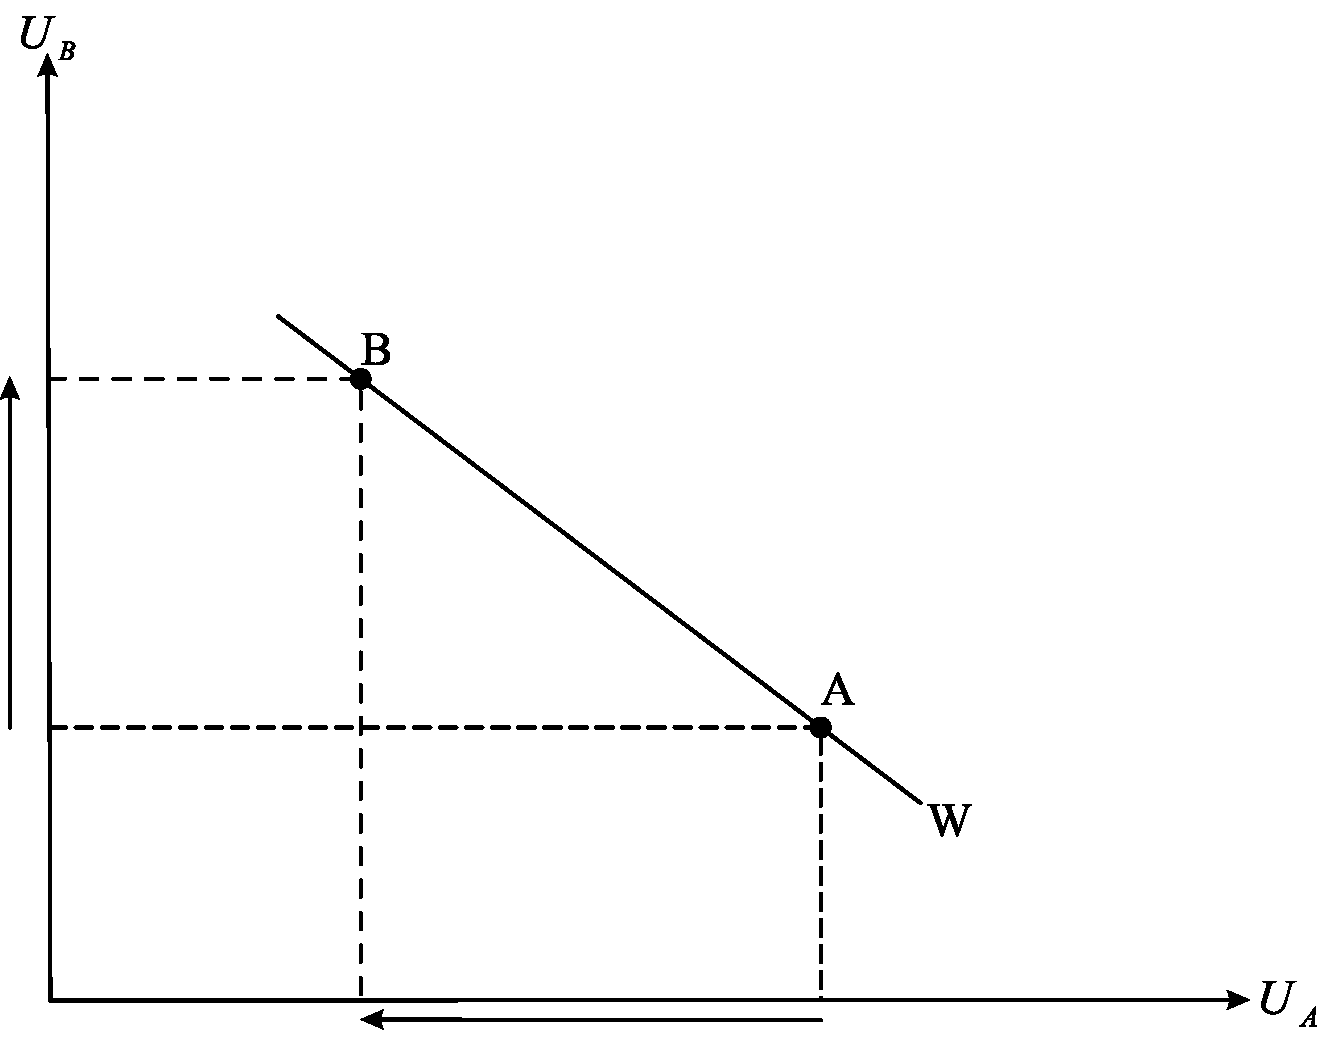
\includegraphics[width = 0.7\linewidth]{figures/fig_09.pdf}
	\end{figure}
\end{frame}
%------------------------------------------------
\begin{frame}{La FBS utilitarista generalizada o convexa}
	\begin{itemize}
		\item Se corresponde con
					$$W(u) = \sum_{i = 1}^{N} g(u_i)$$
		\item Aumentando la concavidad, aumenta la aversión a la desigualdad (característica ausente en la FBS utilitarista pura).
	\end{itemize}
\end{frame}
%------------------------------------------------
\begin{frame}{La FBS utilitarista generalizada o convexa}
Bajo esta forma funcional el \emph{trade off} o tasa de sacrificio entre los diferentes agentes varia según el nivel de sacrificio.
	\begin{figure}[!h]
		\centering
		\hspace{1.2cm}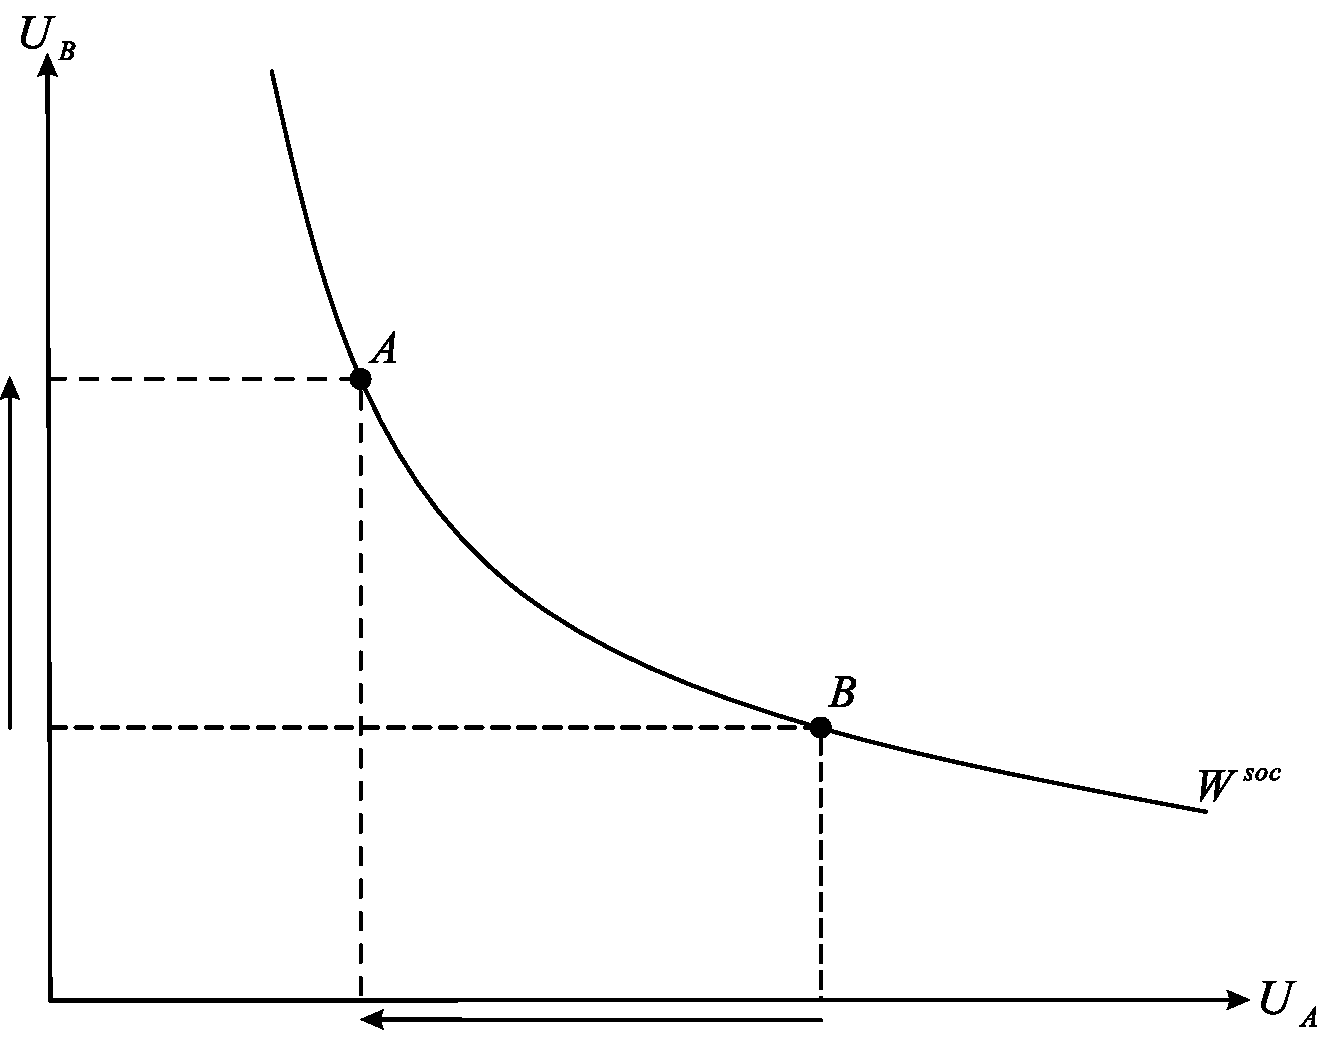
\includegraphics[width = 0.7\linewidth]{figures/fig_10.pdf}
	\end{figure}
\end{frame}
%------------------------------------------------
\begin{frame}{La FBS con aversión a la inequidad}
	\begin{itemize}
		\item Se corresponde con
					$$W(u) = \frac{1}{1-\rho} \sum_{i = 1}^{N} (u_i)^{1-\rho}$$
		\item Siendo la elasticidad de sustitución: $\sigma = \frac{1}{1-\rho}$
		\item Si $\rho = 0$ entonces $\sigma = 1$, se vuelve a la función de Bentham.
		\item Si $\rho$ tiende a infinito entonces $\sigma = 0$, se tiene la función de Rawls
	\end{itemize}
\end{frame}
%------------------------------------------------
\begin{frame}{La FBS maximin o Rawlsiana}
	\begin{itemize}
		\item Se corresponde con
					$$W(u) = \text{min} \left\lbrace u_1, ..., u_N\right\rbrace $$
		\item Optimo social: en aquella alternativa donde el individuo con menos bienestar del grupo mejora.
		\item Se preocupa exclusivamente del bienestar de las personas con mayores necesidades.
	\end{itemize}
\end{frame}